\documentclass[a4paper]{article}

%% Language and font encodings
\usepackage[english]{babel}
\usepackage[utf8x]{inputenc}
\usepackage[T1]{fontenc}

%% Sets page size and margins
\usepackage[a4paper,top=3cm,bottom=2cm,left=3cm,right=3cm,marginparwidth=1.75cm]{geometry}

%% Useful packages
\usepackage{amsmath}
\usepackage{graphicx}
\usepackage[colorinlistoftodos]{todonotes}
\usepackage[colorlinks=true, allcolors=blue]{hyperref}

\title{Evaluacion II}
\author{José Pablo Montaño De la Ree}
\date{26 de Abril 2018}

\begin{document}
\maketitle


\section{Introduction}

En esta evaluacion se modelo el atractor de Lorentz, la cual es un sistema de ecuaciones diferenciales con soluciones caoticas. Para hacer esto se siguio el codigo de Animacion del atractor de Lorentz y de visualizacion de Geoff Boeing. 

\begin{figure}[ht!]
\centering
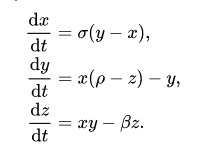
\includegraphics[width=0.3\textwidth]{K.png}
\caption{\label{fig:}}
\end{figure}

\section{Paso 1}

Para inciar se procedio por reproducir el codigo en jupyther lab de la visualizacion y la animacion que ofrece Geoff Boeing. Las graficas obtenidas fueron las siguientes.

\begin{figure}[ht!]
\centering
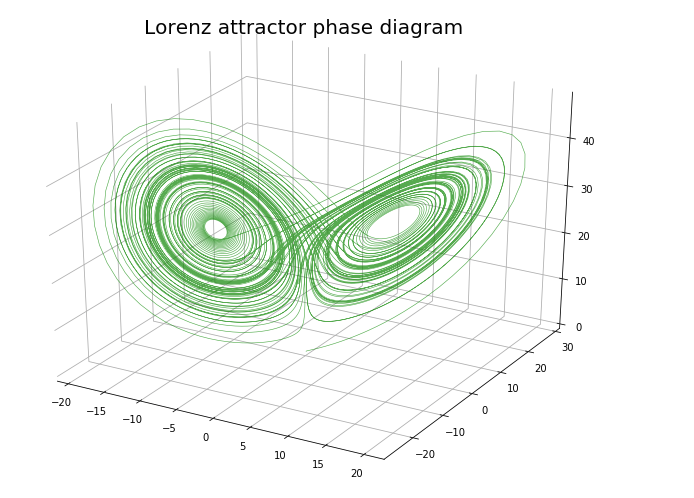
\includegraphics[width=0.3\textwidth]{A1.png}
\caption{\label{fig:}}
\end{figure}

Aqui se puede apreciar la mariposa o infinito que se forma con el atractor de Lorentz en tercera dimension.
\newpage

\begin{figure}[ht!]
\centering
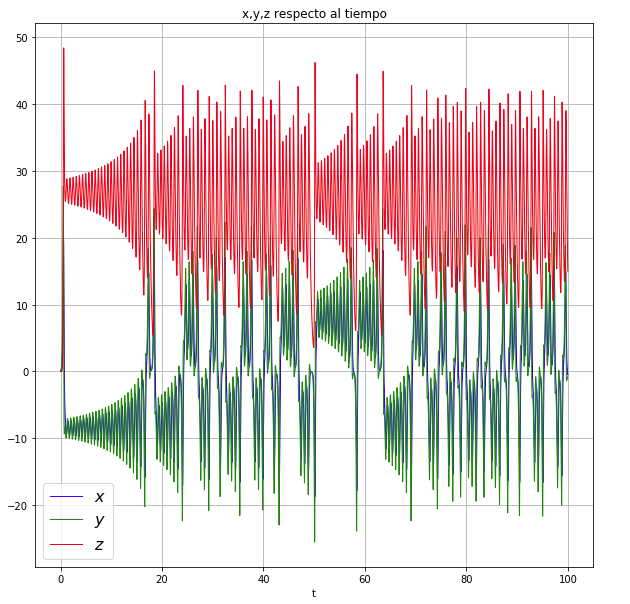
\includegraphics[width=0.3\textwidth]{B1.png}
\caption{\label{fig:}}
\end{figure}

Esta figura muestra la variacion de x, Y, z respecto al tiempo. Para hacer más facil su apreciacion, se muestra la variacion por separado de cada uno de los elemntos antes mecionados. 

\begin{figure}[ht!]
\centering
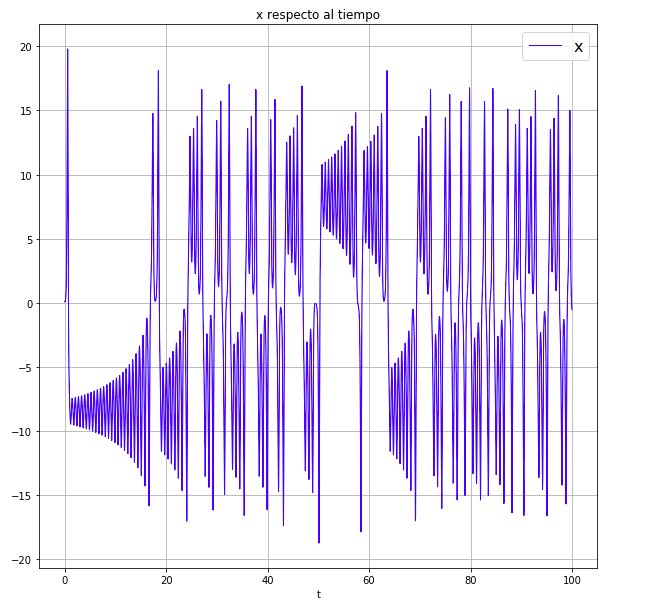
\includegraphics[width=0.3\textwidth]{C1.png}
\caption{\label{fig:}}
\end{figure}

\begin{figure}[ht!]
\centering
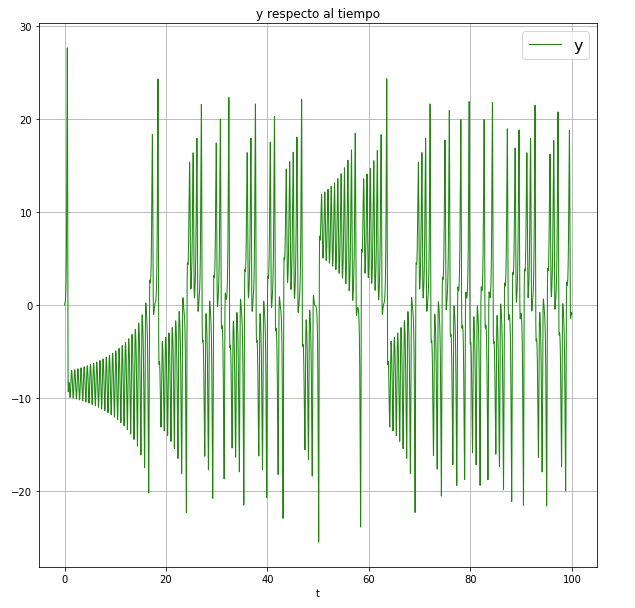
\includegraphics[width=0.3\textwidth]{D1.png}
\caption{\label{fig:}}
\end{figure}

Notese como la figura 4 y 5 se sobreponen y son dificiles de notar en la figura 3. Se podria decir que la variacion de X y Y en este caso es igual.
\newpage

\begin{figure}[ht!]
\centering
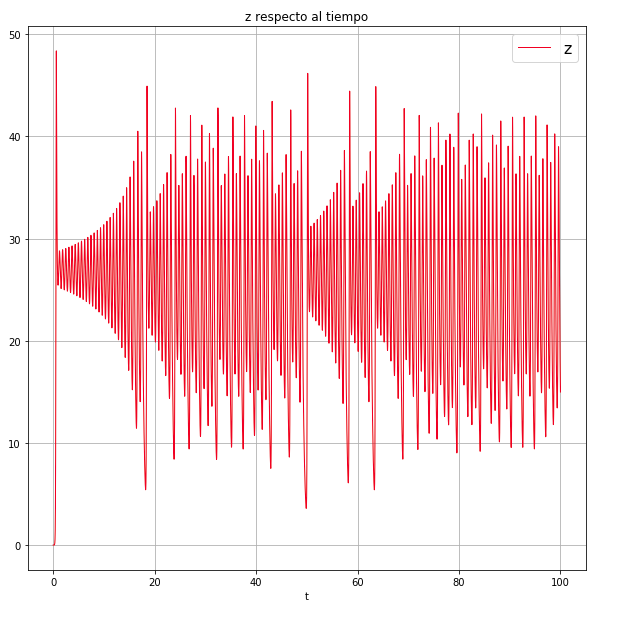
\includegraphics[width=0.3\textwidth]{E1.png}
\caption{\label{fig:}}
\end{figure}

\begin{figure}[ht!]
\centering
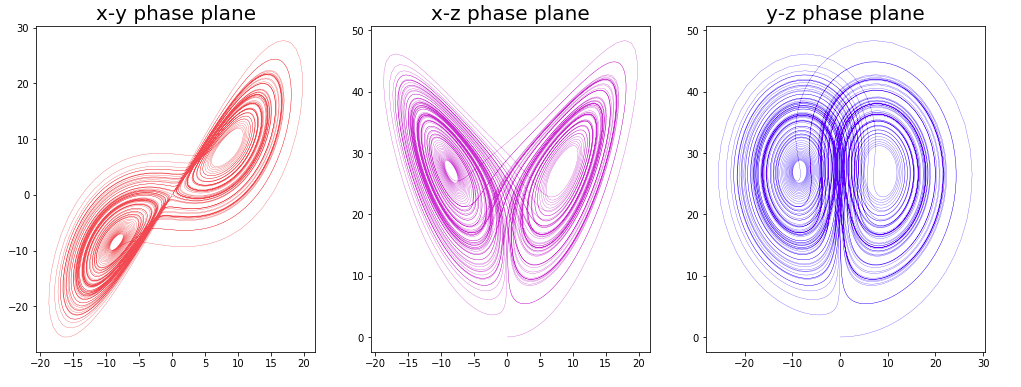
\includegraphics[width=0.3\textwidth]{F1.png}
\caption{\label{fig:}}
\end{figure}
 En estas figuras se puede ver los resultados del atractor de Lorentz en cada uno de los planos. Notese que en planos separados siguen formando "8" o infinitos. 

\section{Paso 2. Graficacion y comparacion}

Despues de haber implementado los codigos de Boeing procedi a realizar calculos para difeentes valores de sigma, beta y rho. Dichos valores eran sigma = 28, beta = 4 and rho = 46.92 y se produjeron las siguientes graficas. 


%%%%%%%%%%%%%%%%%%%%%%%%%%%%%%%%%%%%%%%%%%%%%%%%%%%%%%%%%%%%%%%%%%%%%%%%%%%%
\begin{figure}[ht!]
\centering
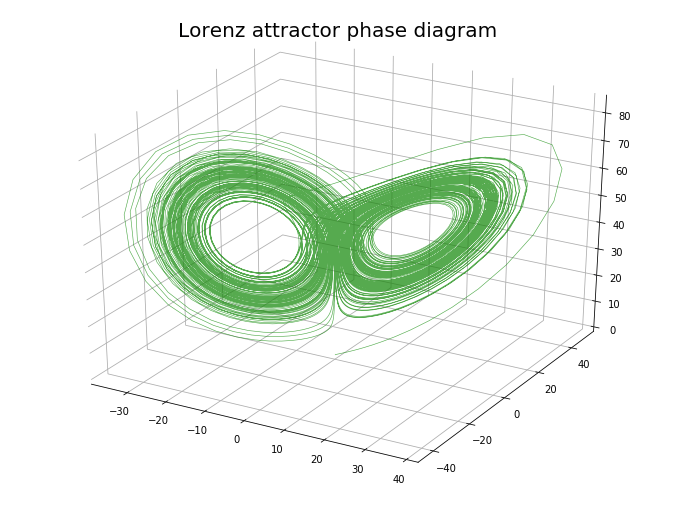
\includegraphics[width=0.3\textwidth]{A2.png}
\caption{\label{fig:}}
\end{figure}

En esta figura de nuevo se puede notar el patron de infinito caracteristico. Sin embargo a acomparacion de la figura 2, esta es mucho más grande y un poco menos erratica.

\newpage

\begin{figure}[ht!]
\centering
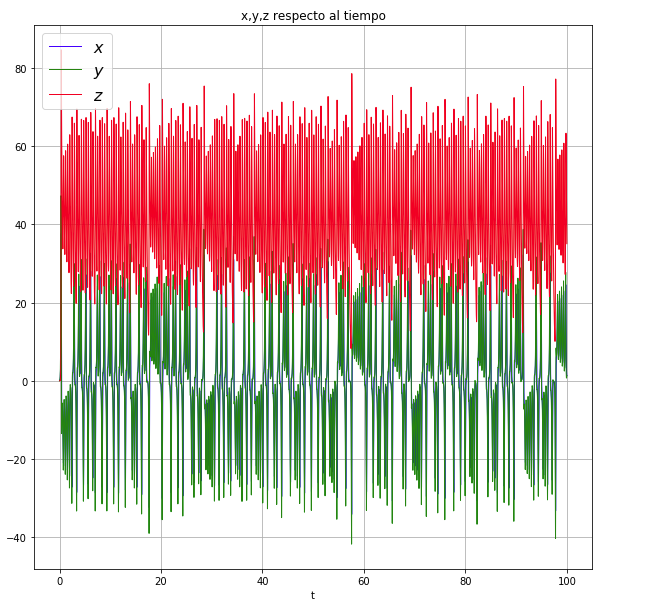
\includegraphics[width=0.3\textwidth]{B2.png}
\caption{\label{fig:}}
\end{figure}

En esta figura se muestra la variacion de X, Y, Z respecto al tiempo. A continuacion se muestan las graficas por separado.  A comparacion de la figura 3, la figura ahora presentada tiene mayor amplitud y es menos erratica que la figura 3.

\begin{figure}[ht!]
\centering
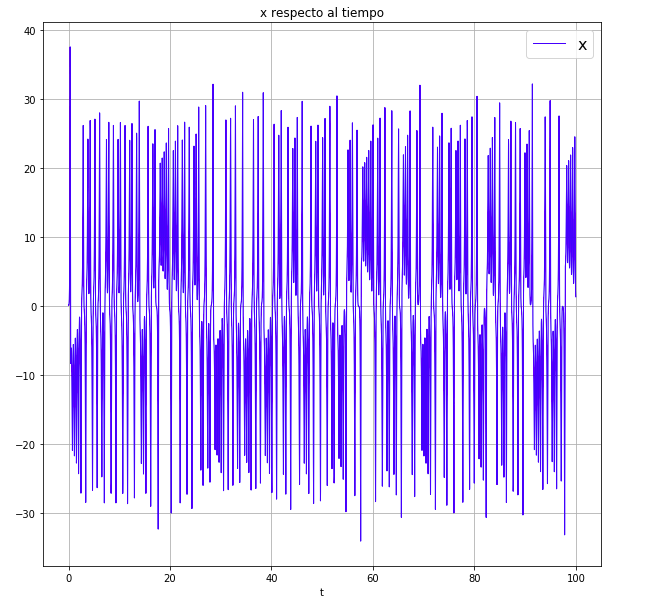
\includegraphics[width=0.3\textwidth]{C2.png}
\caption{\label{fig:}}
\end{figure}

\begin{figure}[ht!]
\centering
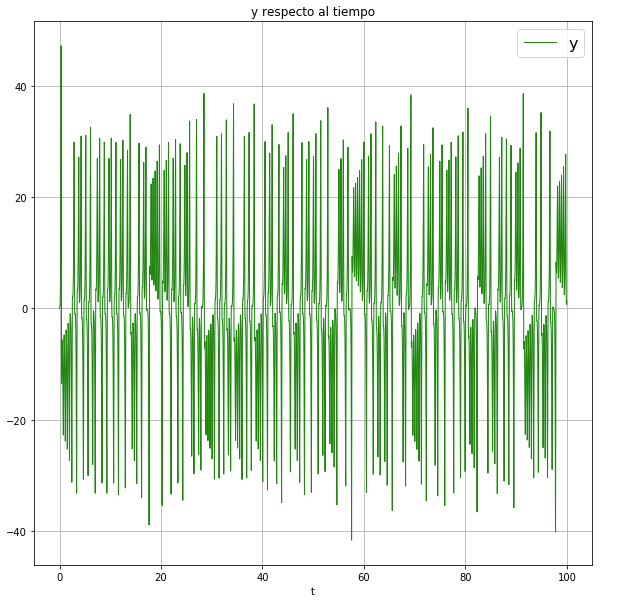
\includegraphics[width=0.3\textwidth]{D2.png}
\caption{\label{fig:}}
\end{figure}

De nuevo estas graficas nos dejan ver como X y Y se comportan de forma similar, al igual que en los casos de la figura 4 y 5 

\begin{figure}[ht!]
\centering
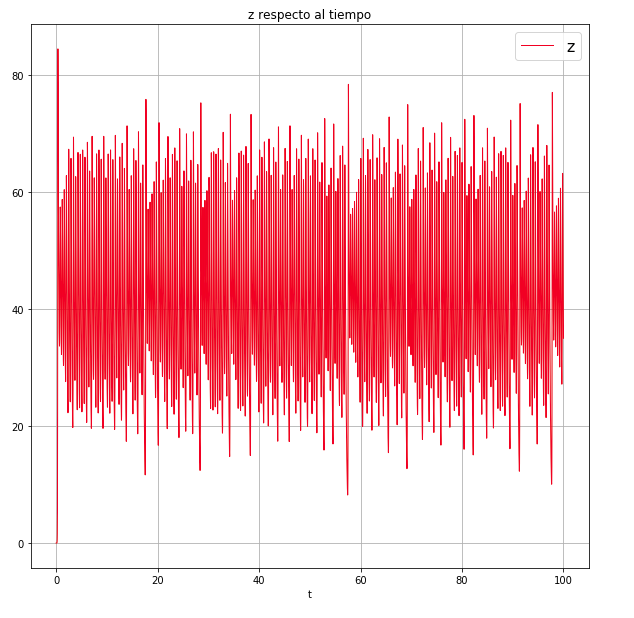
\includegraphics[width=0.3\textwidth]{E2.png}
\caption{\label{fig:}}
\end{figure}
\newpage

Como es de esperarse por lo visto en las graficas anterirores, esta grafica tiene mayor amplitud que la figura 6.   

\begin{figure}[ht!]
\centering
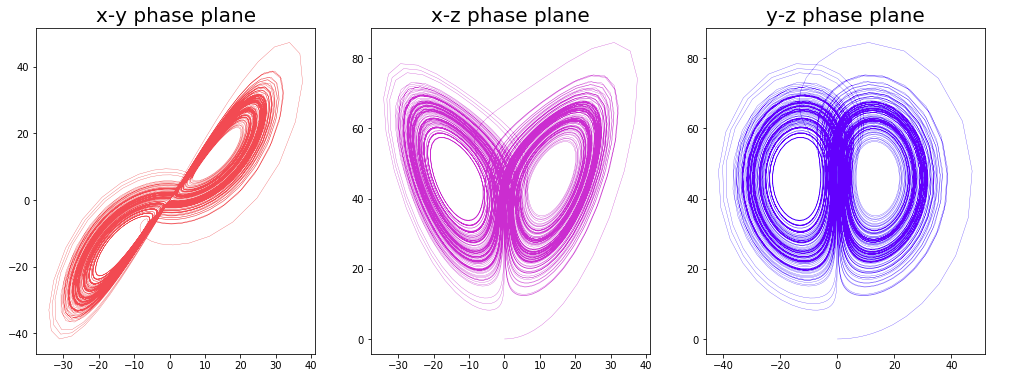
\includegraphics[width=0.3\textwidth]{F2.png}
\caption{\label{fig:}}
\end{figure}

De nuevo se muestran los patrones de infinito y/o maiposa en cada uno de los planos. A comparacion de la figura 7, estos planos se ven más marcados, tiene una amplitud mayor y pareciese que las lineas estan menos separadas unas de otras.  

\section{Parte 4. Graficas y descripcion}

En esta ultima seccion se exploro de la misma forma que ne las secciones anteriorores el comportamiento del atarctor de Lorentz con valores de sigma = 10, beta = 8/3 and rho = 99.96.

%%%%%%%%%%%%%%%%%%%%%%%%%%%%%%%%%%%%%%%%%%%%%%%%%%%%%%%%%%%%%%%%%%%%%%%%%%%%
\begin{figure}[ht!]
\centering
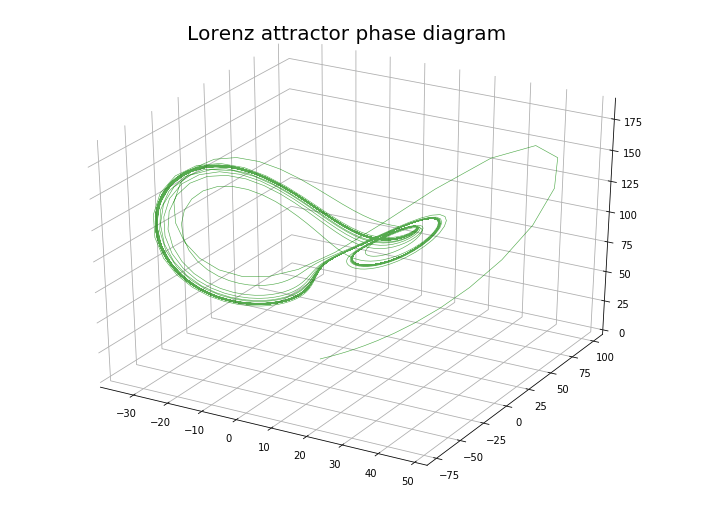
\includegraphics[width=0.3\textwidth]{A3.png}
\caption{\label{fig:}}
\end{figure}

En esta figura se puede apreciar de nuevo la forma de infinito, sin embargo se puede ver que es más erratico que los casos anteriores. De la animacion vista en A2 pareciese que en solo existe un infinito simetrico en ciertas ocaciones del tiempo, pero no se forman al mismo tiempo.

\newpage

\begin{figure}[ht!]
\centering
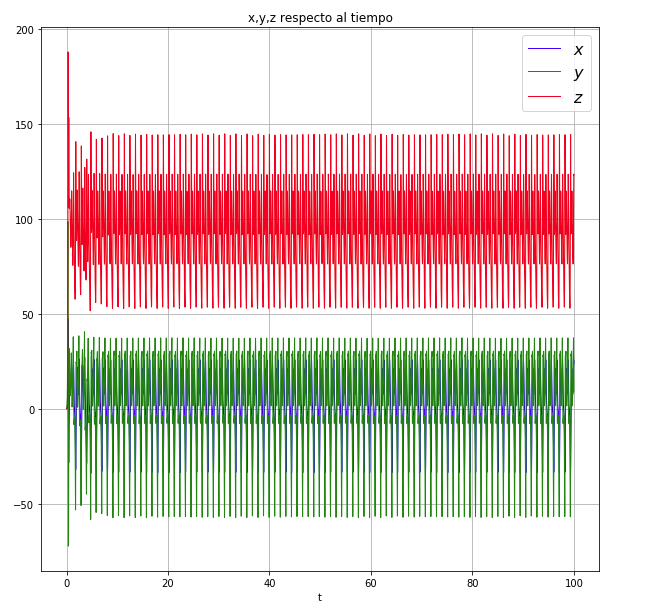
\includegraphics[width=0.3\textwidth]{B3.png}
\caption{\label{fig:}}
\end{figure}

En esta grafica se muestra X, Y y z respecto al tiempo. Notese que pareciese se crean dos secciones, una que contiene a Z en la parte superior y una que contiene a X y Y en la parte inferior.  


\begin{figure}[ht!]
\centering
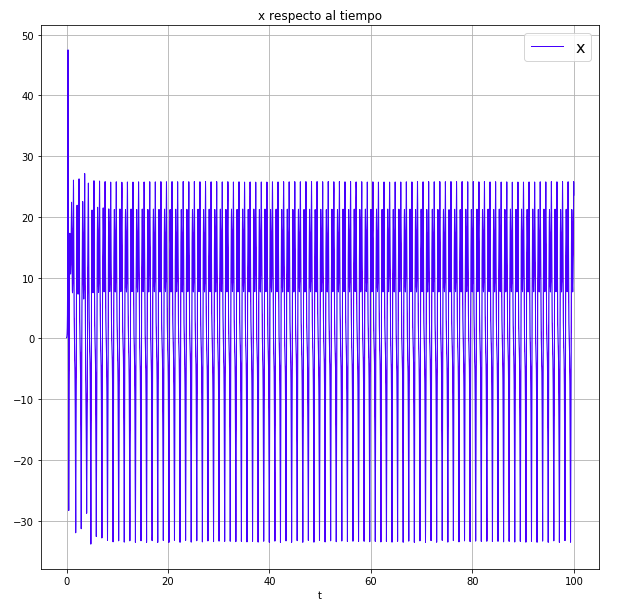
\includegraphics[width=0.3\textwidth]{C3.png}
\caption{\label{fig:}}
\end{figure}

Este es el comportamineto de X respecto al tiempo. Notese que despues de t=5 aproximadamente sus valores no alcanzan el 30. Su rango es de un poco menos de 50 a un poco menos de -30

\begin{figure}[ht!]
\centering
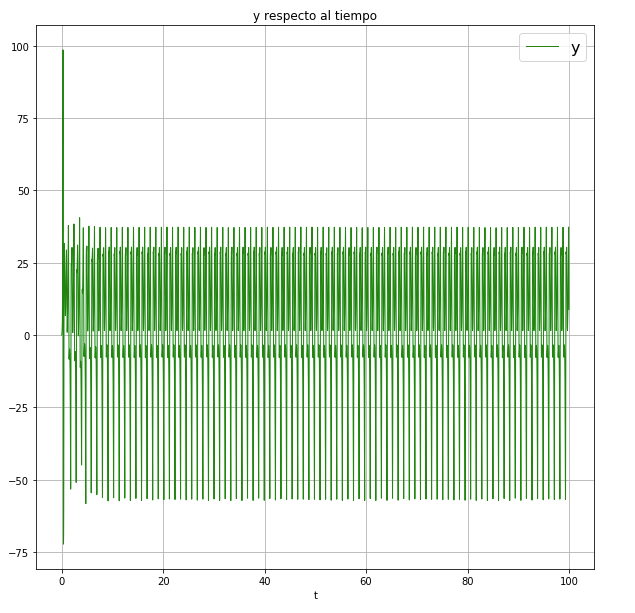
\includegraphics[width=0.3\textwidth]{D3.png}
\caption{\label{fig:}}
\end{figure}

Esta figura muestra el comportamiento de Y respecto al tiempo. Notese que esta tiene un rango que va desde casi 100 hasta casi -75, sin embargo, despues de los primeros segundos su valor pareciera no pasar de 30 tambien al igual que X. Notese que a pesar de comportarse muy similar a X, esta vez no se superponen totalmente. 
\newpage

\begin{figure}[ht!]
\centering
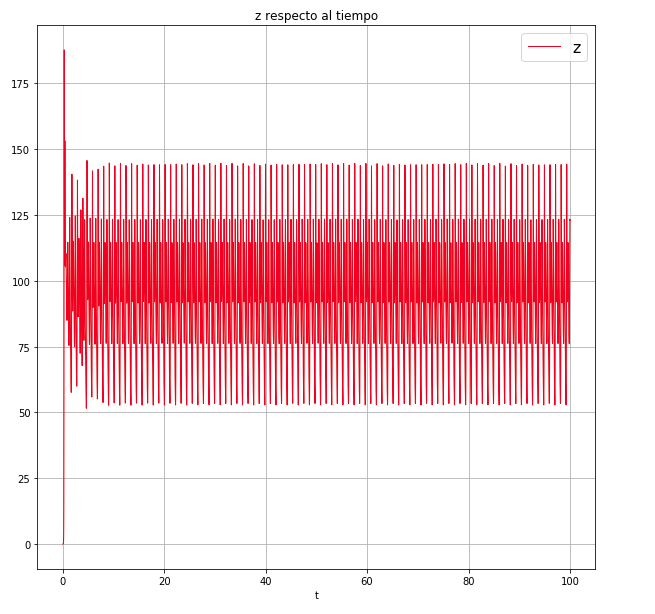
\includegraphics[width=0.3\textwidth]{E3.png}
\caption{\label{fig:}}
\end{figure}


Esta figura muestra la variacion de Z respecto al tiempo. Notese que esta tiene un rango entre 175 y 0, sin embargo despues de los primeros segundos varia entre 150 y 50 aproximadamente, manteniendose alejada de X y Y. 

\begin{figure}[ht!]
\centering
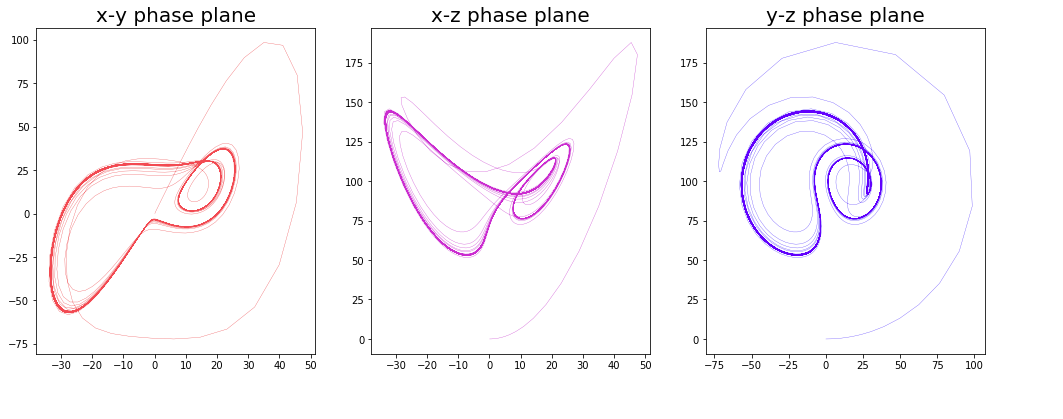
\includegraphics[width=0.3\textwidth]{F3.png}
\caption{\label{fig:}}
\end{figure}

En esta figura podemos apreciar que se forman infinitos aunque no sean tan "obvios" sin  embargo estas figuras son mucho más erraticas a comparacion de las otras realizadas en este trabajo y todas tienen una linea muy alejada del resto de los datos. 

\section{Referencias}

\begin{verbatim}

Geoff Boeing . (2016). lorenz-system-attractor-visualize. 26/4/2018, 
de Github Sitio web: https://github.com/gboeing/lorenz-system
/blob/master/lorenz-system-attractor-visualize.ipynb

Geoff Boeing . (2016). Animated Lorenz Attractor. 26/4/2018,
de Github Sitio web: https://github.com/gboeing/lorenz-system
/blob/master/lorenz-system-attractor-animate.ipynb

Wikipedia. (2018). Lorenz system. 26/4/2018,
de Wikipedia Sitio web: 
https://en.wikipedia.org/wiki/Lorenz_system

\end{verbatim}


\end{document}